\documentclass[conference]{IEEEtran}
% *** GRAPHICS RELATED PACKAGES ***
%
\ifCLASSINFOpdf

\fi
\usepackage{url}
\usepackage[brazilian]{babel}
\usepackage[utf8]{inputenc}
\usepackage[T1]{fontenc}
\usepackage{graphicx}
\usepackage{cite}
\usepackage[pdftex, hidelinks]{hyperref}
\hyphenation{op-tical net-works semi-conduc-tor}

\begin{document}

\title{Simulador de amplificador de áudio}
\author{\IEEEauthorblockN{Paulo Augusto M. F. de Souza}
\IEEEauthorblockA{Estudante de Engenharia Eletrônica\\
Faculdade Gama - FGA UnB\\
Email: pauloaugustomiguelfonseca@gmail.com}
\and
\IEEEauthorblockN{Tiago Martins de Brito}
\IEEEauthorblockA{Estudante de Engenharia Eletrônica\\
Faculdade Gama - FGA UnB\\
Email: tiagomartinsbrito879@gmail.com}
}%final de autores

% make the title area
\maketitle


\begin{abstract}
Com o processamento de sinais de áudio, é possivel modificar as características originais do sinal. Por ser de áudio, pode-se ver o seu comportamento em faixas de frequência diferente e com isso equalizar um sinal da maneira pretendida através de filtros. Também é possível amplificar ele de uma maneira que o torne mais intenso ou menos intenso, modificando a sua amplitude.
\end{abstract}


{\small \textbf{{\textit Palavras-chaves} -- Frequência, filtro, amplificador, equalizador.}}


\IEEEpeerreviewmaketitle



\section{Introdução}
% no \IEEEPARstart
%Equalizar audio, é definir faixas de específicas de frequência.
%Fazer a introdução
 
%\hfill January 11, 2007
\subsection{Justificativa}
Para tratamento de sinais de áudio com equipamentos digitais ou analógicos, ainda há um elevado custo, então como esse projeto tem como motivação tentar reduzir esses custos, mas tendo em vista manter uma certa qualidade. Com esse custo reduzido, poderia ser usado para o aprendizado para quem ainda está aprendendo e não quer gastar muito com equipamentos de áudio. 

\subsection{Objetivos}
O objetivo deste trabalho, é mostrar como pode ser feita a equallização de áudio, com o Raspberry Pi através da amostragem de um sinal. 

\subsection{Requisitos}
A priori está sendo estudada a possibilidade de usar um conversor AD, de pelo menos 16 bits e uma frequência de amostragem de 40kHz, ou no lugar dele colocar uma interface de áudio, que tem uma taxa de amostragem de 48kHz e de 24 bits. Isso se deve pois o Raspberry não possui conversor AD, então é preciso usar um externo. 

Sensores serão usados para colocar algum tipo de efeito durante o processamento do sinal pelo Raspberry, como por exemplo um sensor de distância para colocar a intensidade do efeito. Também pode ser adicionado um VU-Meter, para mostrar as bandas de frequência do sinal. 

Para todos os cálculos e processamentos dos sinais, será usado o Raspberry Pi 3. Ele será usado pois, tem uma grande capacidade de processamento, e com uma boa velocidade. O uso dele permite criar sistemas embarcados para essa aplicação de processamento de sinais de áudio.


\section{Revisão Bibliográfica}
\subsection{Teorema da amostragem}
Para o processamento computacional de um sinal analógico, antes é preciso fazer a amostragem do sinal. Isso consiste em discretizar o sinal, ou seja, torna-lo digital e com isso fazer o seu processamento em um computador, ou no Raspberry Pi. Amostrar é definir para um certo intervalo de tempo, um valor para o sinal. Onde esse ele apenas possui um valor definido em um intervalo de tempo específico.

\begin{figure}[!h]%h = here
\centering

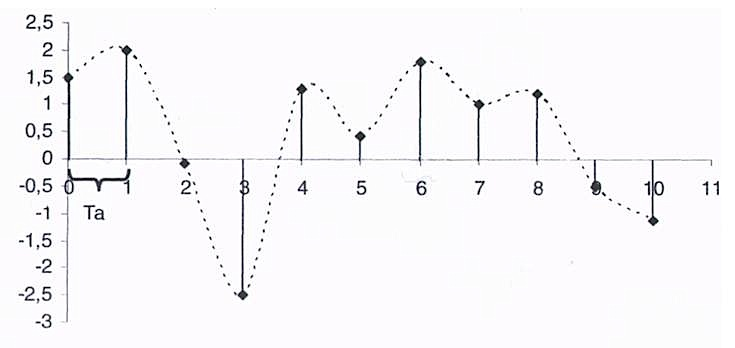
\includegraphics[width=2.5in]{Imagens/amostragem1} %define a largura como 2.5 polegagas
\caption{Amostragem}
%\flushleft{\small 
%Fonte: \url{https://susanasousa.wordpress.com/2011/01/23/audio-digital-frequencia-de-amostragem}}

\label{amos}
\end{figure}

Na Figura \ref{amos}, é possível ver justamente, onde para cada intervalo de tempo é que se tem uma amostra do sinal, um valor definido apenas em um intervalo de tempo específico. Em intervalos de tempo não definido, o sinal recebe zero como seu valor.

Um meio para as discretização, é usar o critério de Nyquist para amostragem, que diz que a frequência de amostragem deve ser de pelo menos duas vezes a frequência do sinal. Isso se deve para que se possa retomar o sinal original com o mínimo de distorções possíveis. 
Na Figura \ref{fig_sim} é possivel ver justamente esse critério, pois quando a frequência de amostragem é duas vezes menor, há uma sobreposição do sinal, e isso não permite voltar ao sinal original. \cite{mello2013processamento}

\begin{figure}[!htb]
\centering
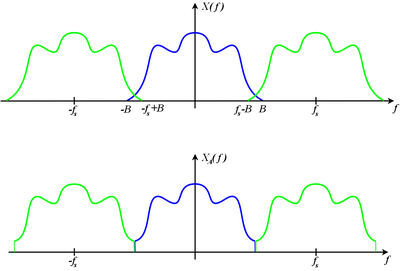
\includegraphics[width=2.2in, height = 1.2in]{Imagens/nyquist}
\caption{Nyquist}
\flushleft{\small 
Fonte: \url{https://pt.wikipedia.org/wiki/Teorema_da_amostragem_de_Nyquist-Shannon}}

\label{fig_sim}
\end{figure}

\subsection{Processamento de sinais}

Em áudio a largura de banda corresponde ao espectro audível, compreendido entre 20 e 20kHz. %citação aqui ppgee.ufmg.br/defesas/486M-PDF
Então, a partir de dispositivos de captação sonora, o objetivo é trabalhar com faixas de frequência compreendidas na parte audível. Com isso, se busca então trabalhar com a resposta em frequência dessa faixa.
\cite{herrera2004projeto}

O processamento desses sinais, podem ser feitos com a aplicação de filtros, que delimitam uma faixa específica para se trabalhar. Esses filtros, que podem ser, passa baixas, passa altas ou passa bandas, servem para fazer a equalização de um sinal de áudio. Além dessa equalização, também podem ser incorporados controles para ajuste da amplitude dos sinais antes e após o processamento.
\cite{ferreira2014processamento}

Filtros passa baixas, são dispositivos que permitem a passagem de um sinal até uma certa frequência máxima. Passa altas, são os que permitem a passagem a partir de uma frequência mínima. E passa bandas, são os que permitem a passagem a partir de uma frequência mínima até uma máxima. As figuras abaixo mostram justamente a resposta em frequência de cada filtro.

%%%%%%%%%%%%%%%%%%%%%%%%%%%%%%%%%%%%%%%%%%%%%%

%imagens de filtros
%Passa-Baixas
\begin{figure}[!h]
\centering
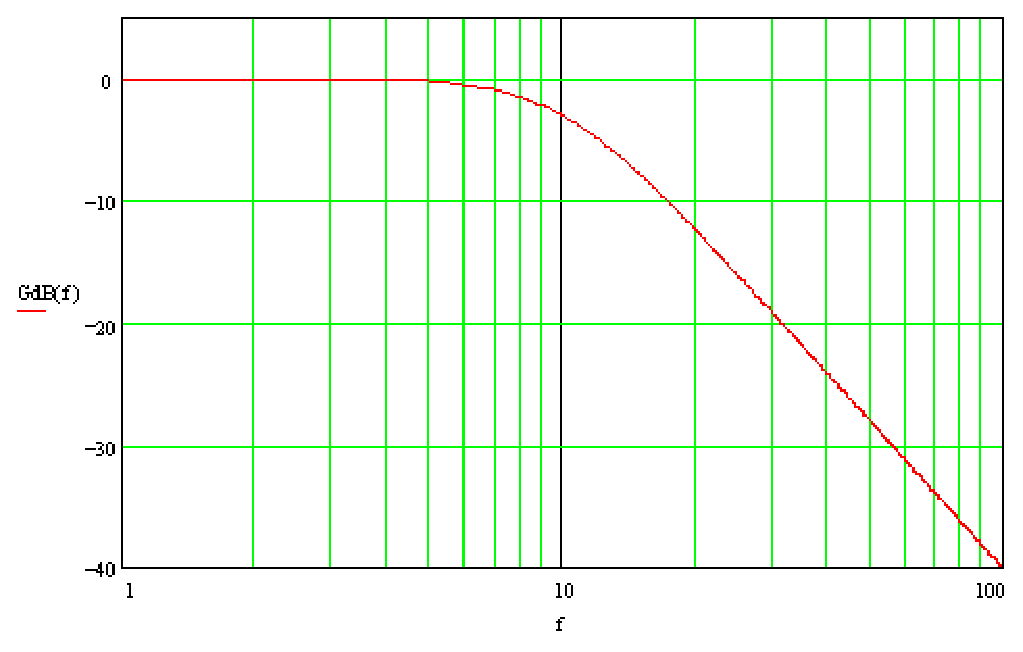
\includegraphics[width=2.5in, height=1.1in]{Imagens/baixass.eps}
\caption{Passa baixas} 
\flushleft{\small 
Fonte: \url{http://www.alvaroneiva.site.br.com/filteq2_arquivos/image011.gif}}
\label{baixa}
\end{figure}
%Passa-Bandas
\begin{figure}[!htb]
\centering
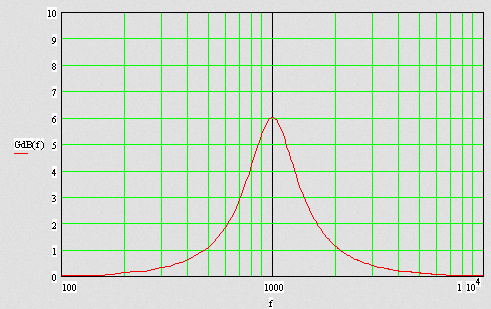
\includegraphics[width=2.5in, height=1.1in]{Imagens/BANDAA.png}
\caption{Passa banda}
\flushleft{\small 
Fonte: \url{http://www.alvaroneiva.site.br.com/filteq2_arquivos/image015.gif}}
\label{banda}
\end{figure}
%Paassa-Altas
\begin{figure}[!htb]
\centering
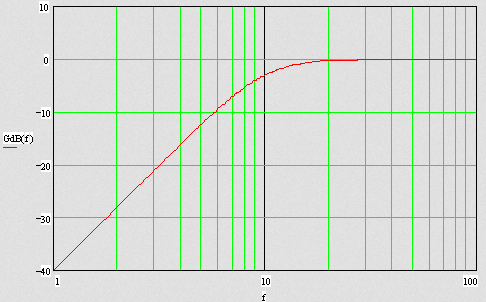
\includegraphics[width=2.5in, height=1.1in]{Imagens/ALTAA.png}
\caption{Passa alta} 
\flushleft{\small 
Fonte: \url{http://www.alvaroneiva.site.br.com/filteq2_arquivos/image013.gif}}
\label{alta}
\end{figure}


\section{Desenvolvimento}

A primeira parte do desenvolvimento, foi conectar a interface de áudio Roland DuoCapture UA11 ao Linux. 
Essa conectividade foi possível com a entrada P10 da interface, pois quando tentamos usar o P2 não foi possível gravar um arquivo de áudio. A gravação, foi possível usando um software para esse tipo de tarefa, o Ardour, e também um que já vem na Raspberry Pi, o Alsamixer.

Após a gravação, é possível ouvir o áudio gravado, com o Ardour, na saída da interface. Quando a gravação é feita usando o Alsamixer é possível ouvir o som na saída P2 da Raspberry Pi ou via o audio da saída HDMI. 

Após a leitura, o próximo passo então é fazer o processamento desse sinal de áudio, adicionar efeitos e aplicar filtros para tratamento sinal recebido na Raspberry. Esses filtros podem ser desenvolvidos na Raspberry e com isso modificar o sinal para que possa ser percebido as diferenças na saída. Com isso, embarcar o sistema utilizando alguns sensores, como o de presença até o momento mencionado.

\subsection{Descrição de Hardware}

A ligação da interface com a Raspberry Pi é feita através do cabo USB que permite a sua comunicação. O instrumento é conectado na interface de áudio para que seja feito uma conversão AD para que seja possível a leitura e gravação dos dados. 

A conecção do instrumento pode ser feita com o conector de entrada P10 da interface permitindo assim que ela faça a conversão AD. Como essa interface possui uma taxa de amostragem de 48KHz, a qualidade do sinal audível é muito boa, assim é possível fazer uma análise mais robusta do áudio e consequentemente o seu processamento, enfatizando algumas informações extraidas através de filtros, permitindo que sinais semelhantes ao de um simulador de amplificador de guitarra sejam executados como saída do sistema.

\begin{figure}[!htb]
\centering
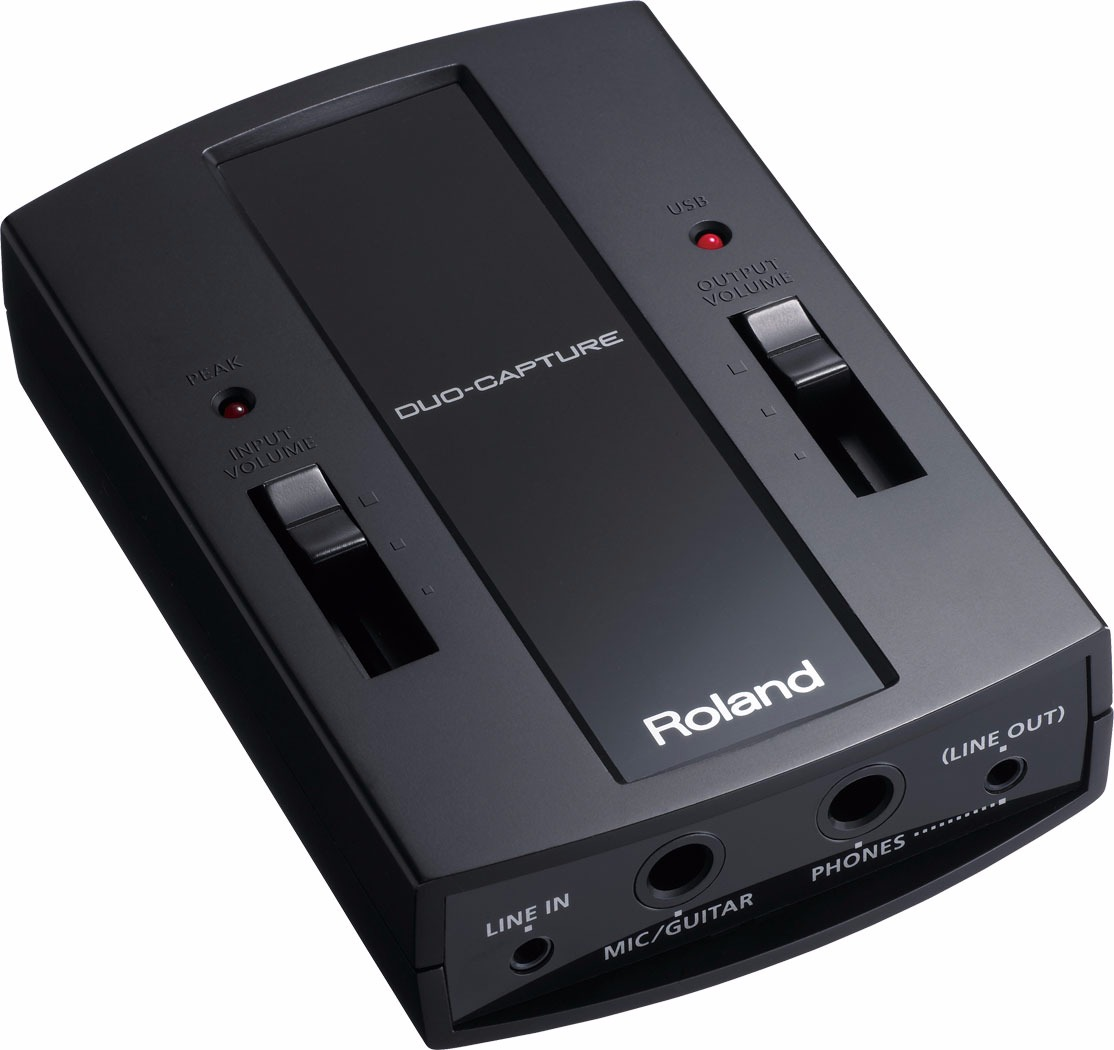
\includegraphics[width=2.5in, height=2.2in]{Imagens/interface}
\caption{Interface de áudio} 
\flushleft{\small 
Fonte: \url{https://www.roland.com/us/products/duo-capture/}}
\label{interface}
\end{figure}

A Figura \ref{interface} traz a interface de áudio usada para nosso projeto. Nela contém duas entradas e duas saídas, assim é possível conectar mais de um equipamento para gravação. E atrás dela possui o conector para se ligar o cabo USB para ser feita a conexão com o computador ou a Raspberry Pi.

\begin{figure}[!htb]
\centering
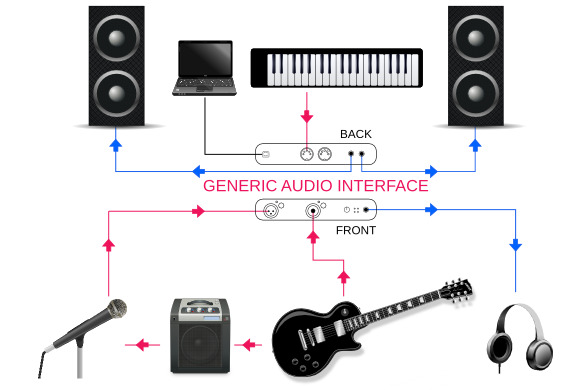
\includegraphics[width=3.0in, height=2.2in]{Imagens/conection}
\caption{Conecção da interface e o PC} 
\flushleft{\small 
Fonte: \url{http://libremusicproduction.com/sites/default/files/articles/Bedroom\%20musician\%20setup.png}}
\label{conection}
\end{figure}

Na Figura \ref{conection} é possível ver como ele pode ser ligado ao computador ou ao Raspberry Pi. Esse tipo de interface permite que não apenas um tipo de instrumento ou microfone possa ser ligado a ela.

Esse tipo de implementação de hardware permite que se faça então a leitura do PC ou da Raspberry do sinal que pode ser tratado e então enviado para saídas de áudio e então ser escutado por uma pessoa através de um fone ou auto falante.

%%%%%%%%%%%%%%%%%%%%%%%%%%%%%%%%%%%%%%
%%%%%%%%%%%NOVAS FIGURAS%%%%%%%%%%%%%%
\begin{figure}[!htb]
\centering
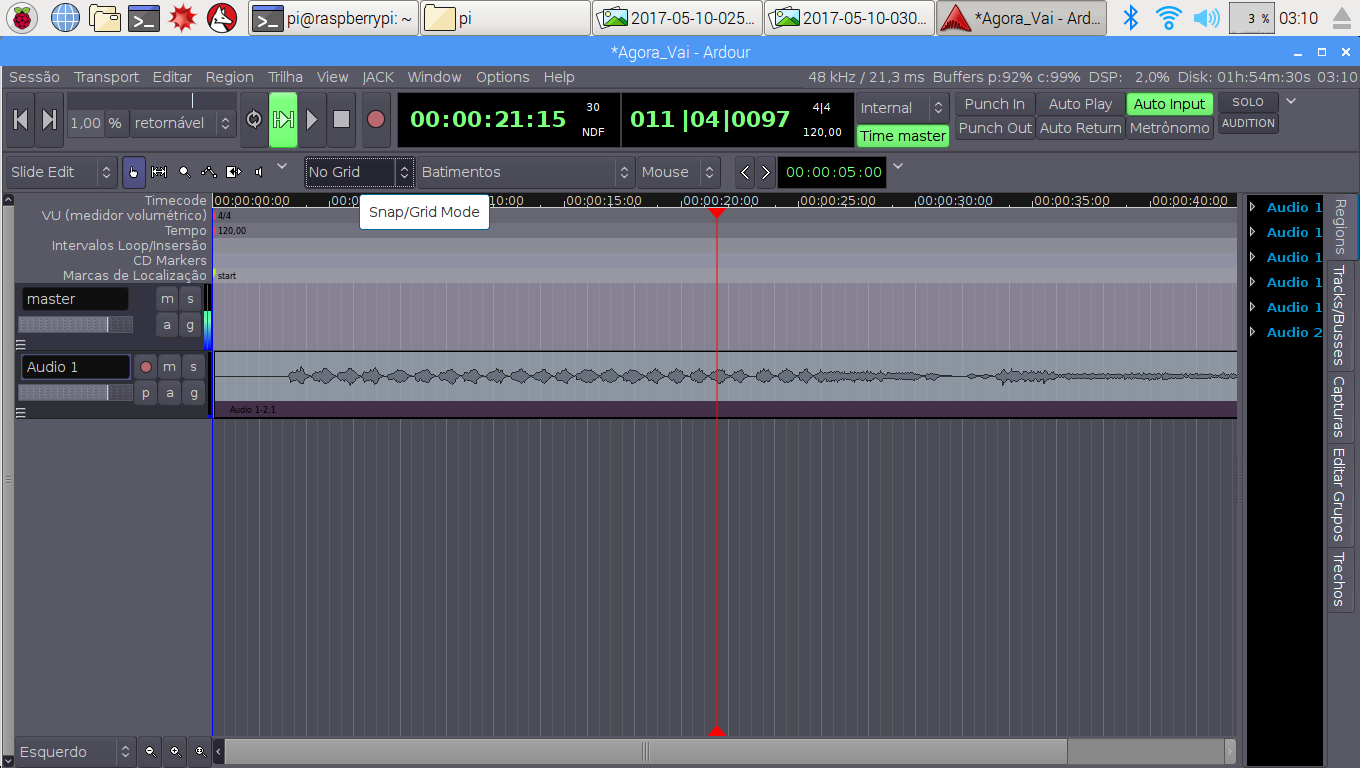
\includegraphics[width=3.5in, height=2.2in]{Imagens/Simulacao_Ardour2}
\caption{Teste de Gravação} 
\flushleft{\small 
Fonte: extraído diretamente pela Raspberry Pi 3-B}
\label{Simulacao_Ardour}
\end{figure}

Na figura \ref{Simulacao_Ardour} foi realizado uma gravação de teste, usando o software Ardour implementado na raspberry pi 3-B, cujo foi instalado na placa.

Para a gravação foi utilizado um mini teclado (instrumento) SA-46 da CASIO, a gravação saiu como o esperado e foi realizada com o ganho em 50\% tanto do instrumento (OUTPUT) quanto da interface de audio (da INPUT).

\begin{figure}[!htb]
\centering
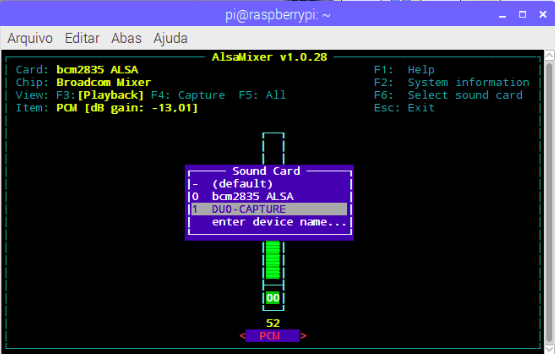
\includegraphics[width=3.5in, height=3in]{Imagens/Alsamixer}
\caption{Conecção da interface e o PC} 
\flushleft{\small 
Fonte: extraído diretamente pela Raspberry Pi 3-B}
\label{Alsamixer}
\end{figure}

Na figura \ref{Alsamixer} mostra que a interface UA-11 Duo-Capture da Roland foi reconhecida e selecionada para gravação. Abaixo na figura \ref{amixer} é possível observar os comandos utilizados para gravação “arecord -D plughw:1,0 test.wav” e "ctrl+c" usado para parar a gravação, posteriormente o comando “aplay test.wav” para ouvir a gravação através do JACKda raspiberry ou da saída de áudio via HDMI.
\begin{figure}[!htb]
\centering
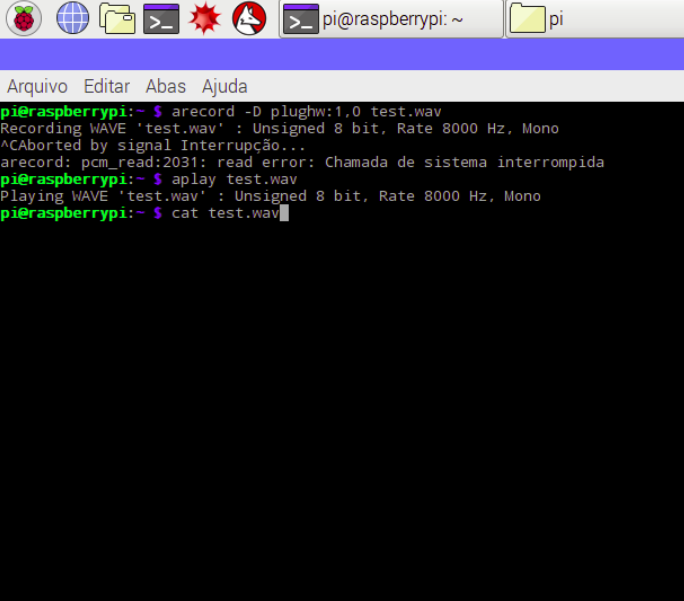
\includegraphics[width=3.5in, height=3in]{Imagens/amixer}
\caption{Conecção da interface e o PC} 
\flushleft{\small 
Fonte: extraído diretamente pela Raspberry Pi 3-B}
\label{amixer}
\end{figure}
\\
%%%%%%%%%%%%%%%%%%%%%%%%%%%%%%%%%%%%%%%%%%

\subsection{Descrição de Software}

\begin{flushleft}

\textbf{Implementação do Filtro passa-baixas}
\end{flushleft}
 
%MUDAR!!! duas primeiras linhas
Foi realizada uma tentativa de implementar um filtro passa baixa usando média móvel. Para isso abriu-se um arquivo de áudio dentro de um programa em C, copiou-se as amostras deste arquivo e essas amostras foram coladas em um outro arquivo de audio com o filtro implementado. 
Contudo esse tipo de implementação não é a esperada para o projeto que visa uma tentativa de fazer o processamento do sinal em tempo real. Esse tipo de tentativa foi feita pelo motivo de não conseguir ler as amostras vindas da  interface de audio via usb. O código usado para o filtro passa-baixas com médias móveis é da Figura \ref{codigo}:

\begin{figure}[!htb]
\centering
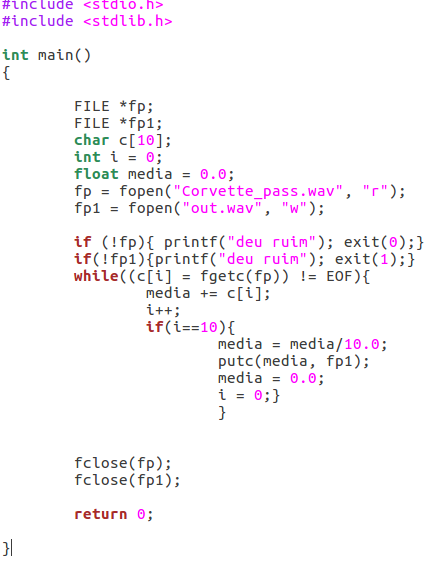
\includegraphics[width=2.5in, height=4in]{Imagens/vai}
\caption{Código usado como tentantiva de implementação} 
\label{codigo}
\end{figure}

O código começa abrindo um arquivo de áudio (.wav), apenas para leitura e outro para escrita. Foi feito a leitura desse arquivo posição por posição e então gravado em um caractere "c". Realizou-se a soma desses caracteres para calcular a média entre eles com 10 caracteres. 
Essa foi a lógia usada para fazer um filtro com médias móveis. No entanto, o problema apresentado aqui é que se faz necessário gravar primeiro o arquivo de áudio (um sinal de áudio) e depois processar o arquivo. Mas o propósito do nosso projeto é tentar implementar esse processo em tempo real, criando assim um equalizador. Porém, esta foi a tentativa realizada nesse ponto de controle.
\\
\bibliographystyle{plain}

\bibliography{Referencias}


% that's all folks
\end{document}


\grid
